\documentclass[pdf,xcolor={dvipsnames}]{beamer}
\usepackage{xcolor,soul}

\makeatletter
\newcommand\hcol{%
	\let\set@color\beamerorig@set@color
	\let\reset@color\beamerorig@reset@color}
\newcommand\tcol{\usebeamercolor[fg]{frametitle}}
\newcommand\red{\color{red}}
\makeatother

\mode<presentation>{\usetheme{default}}
\title{An Efficient Exact Solution to the \newline ($l$,$d$) Planted Motif Problem}
\author{Maria Clara Isabel Sia*\\Julieta Nabos\\Proceso Fernandez}

\begin{document}
\begin{frame}\titlepage\end{frame}

\begin{frame}{Context of the problem}{($l,d$) planted motif problem}
	\only<1>{
		\begin{itemize}
		\item {\tcol DNA motif finding}: known as a difficult (NP-complete) problem in computational biology and computer science\\\ \\
		\item {\tcol motifs}: important sequences that occur repeatedly (but not cleanly, due to mutation) in DNA\\\ \\
		\item {\tcol ($l,d$) planted motif problem}: search for a common motif of length $l$, allowing for up to $d$ mismatches due to mutation.\\\ \\
		\end{itemize}
	}
	\only<2>{
		\centering
		\emph{Find a motif of length {\tcol $l$=8} across these DNA sequences.}\\
		\emph{Each contains the motif with at most {\tcol $d$=2} mismatches.}\\\ \\
		\small
		$\tcol S_1$\ \ \ \texttt{at{cactcgtt}ctcctctaatgtgtaaagacgtactaccgacctta}\ \ \ \ \ \ \\\ \\

		$\tcol S_2$\ \ \ \texttt{acgccgaccggtcccatccttgtatagctcctaacgggcatcagc}\ \ \ \ \ \ \\\ \\
		
		$\tcol S_3$\ \ \ \texttt{tcctgactgcatcgcgatctcggtagtttcctgttcatcattttt}\ \ \ \ \ \ \\\ \\

		$\tcol S_4$\ \ \ \texttt{ggccctcagcatcgtgcgtcctgctaacacattcccatgcagctt}\ \ \ \ \ \ \\\ \\
		
		$\tcol S_5$\ \ \ \texttt{tgaaaagaatttacggtaaaggatccacatccaatcatttgaaag}\ \ \ \ \ \ \\\ \\\ \\

		\emph{Planted motif: }\texttt{\ \ \ ?\ ?\ \ \ \ }\\
	}
	\only<3>{
		\centering
		\emph{Find a motif of length {\tcol $l$=8} across these DNA sequences.}\\
		\emph{Each contains the motif with at most {\tcol $d$=2} mismatches.}\\\ \\
		\small
		$\tcol S_1$\ \ \ \texttt{at\hcol\hl{c{\red\bf ac}tcgtt}ctcctctaatgtgtaaagacgtactaccgacctta}\ \ \ \ \ \ \\\ \\

		$\tcol S_2$\ \ \ \texttt{acgccgaccggtc\hcol\hl{ccatc{\red\bf c}tt}gtatagctcctaacgggcatcagc}\ \ \ \ \ \ \\\ \\

		$\tcol S_3$\ \ \ \texttt{tcctgactgcatcgcgatctcggtagtttcctgt\hcol\hl{{\red\bf t}catc{\red\bf a}tt}ttt}\ \ \ \ \ \ \\\ \\

		$\tcol S_4$\ \ \ \texttt{ggccctca\hcol\hl{{\red g}catcgt{\red\bf g}}\color{black}cgtcctgctaacacattcccatgcagctt}\ \ \ \ \ \ \\\ \\
		
		$\tcol S_5$\ \ \ \texttt{\color{black}tgaaaagaatttacggtaaaggatccacatc\hcol\hl{c{\red\bf a}atc{\red\bf a}tt}tgaaag}\ \ \ \ \ \ \\\ \\\ \\

		\color{black}{\em Planted motif: }\texttt{\hcol\hl{ccatcgtt}}\\
	}
	\end{frame}


\begin{frame}{Key concepts}{($l,d$) planted motif problem}
	\begin{itemize}
		\item an {\tcol $l$-mer} is a sequence of length $l$
		\item two $l$-mers are {\tcol $d$-neighbors} if they have at most $d$ mismatches\\\vspace*{4pt}
		% \item the number of mismatches is called the {\tcol Hamming distance, $d_H$}\\\vspace*{4pt}
		\begin{columns}
			\begin{column}{0.15\textwidth}\end{column}
			\begin{column}{0.2\textwidth}
				$l$=8,\ $d$=3,
			\end{column}
			\begin{column}{0.45\textwidth}
			\begin{center} {
				$x_1$ = \texttt{c{\color{red}g}atc{\color{red}c}tt}\\
				$x_2$ = \texttt{c{\color{red}c}atc{\color{red}g}tt}\\
			}\end{center}
			\end{column}
			\begin{column}{0.3\textwidth}
			% \begin{center} {
				$d_H(x_1,x_2) = 2$\ \ \\
			% }\end{center}
			\end{column}
			\begin{column}{0.1\textwidth}\end{column}
			\end{columns}\ \\\vspace*{4pt}
		\end{itemize}
	% \color{black}
	% {\centering Given a set $\mathcal{S} = \{S_{1},...S_{n}\}$ of $n$ DNA sequences,\\\vspace*{4pt}
	% find $M$, the set of all {\tcol $l$-mers} (sequences of length $l$)\\\vspace*{4pt}
	% which have at least one {\tcol $d$-neighbor} in each sequence in $S$.\\\ \\\vspace*{4pt}}
	% \only<1>{\begin{itemize}
	% 	\item two $l$-mers are {\tcol $d$-neighbors} if they have at most $d$ mismatches\\\vspace*{4pt}
	% 	% \item the number of mismatches is called the {\tcol Hamming distance, $d_H$}\\\vspace*{4pt}
	% 	\begin{columns}
	% 		\begin{column}{0.15\textwidth}\end{column}
	% 		\begin{column}{0.2\textwidth}
	% 			$l$=8,\ $d$=3,
	% 		\end{column}
	% 		\begin{column}{0.45\textwidth}
	% 		\begin{center} {
	% 			$x_1$ = \texttt{c{\color{red}g}atc{\color{red}c}tt}\\
	% 			$x_2$ = \texttt{c{\color{red}c}atc{\color{red}g}tt}\\
	% 		}\end{center}
	% 		\end{column}
	% 		\begin{column}{0.3\textwidth}
	% 		% \begin{center} {
	% 			$d_H(x_1,x_2) = 2$\ \ \\
	% 		% }\end{center}
	% 		\end{column}
	% 		\begin{column}{0.1\textwidth}\end{column}
	% 		\end{columns}\ \\\vspace*{4pt}
	% 	\end{itemize}
	% 	}
	% \only<2->{\begin{itemize}
	% 	\item {\tcol heuristic algorithms} do an iterative local search for motifs
	% 	\begin{itemize}\item ex. sampling and projection---quick, but non-exhaustive\\\ \\\end{itemize}
	% 	\item {\tcol exact algorithms} do an exhaustive search for motifs
	% 	\begin{itemize}
	% 		\item ex. combinatorics---finds all possible motifs, but time-intensive
	% 		\end{itemize}	
	% 	\end{itemize}
	% 	}
	\end{frame}

\begin{frame}{EMS-GT}{EMS-GT}
	\begin{itemize}
	\item we developed an {\tcol exact motif search} (EMS) algorithm 
		  that uses the candidate {\tcol generate-and-test} (GT) approach\\\ \\
	% \item EMS-GT efficiently solves any ($l,d$) planted motif problem instance for $l \leq 17$\\\ \\
	\item {\tcol generate} - narrow down the search to a set of candidate motifs
	\item {\tcol test} - check each candidate to determine if it is a motif
	\end{itemize}
	\end{frame}

\begin{frame}{Demonstration of algorithm}{EMS-GT}
	\only<1>{\centering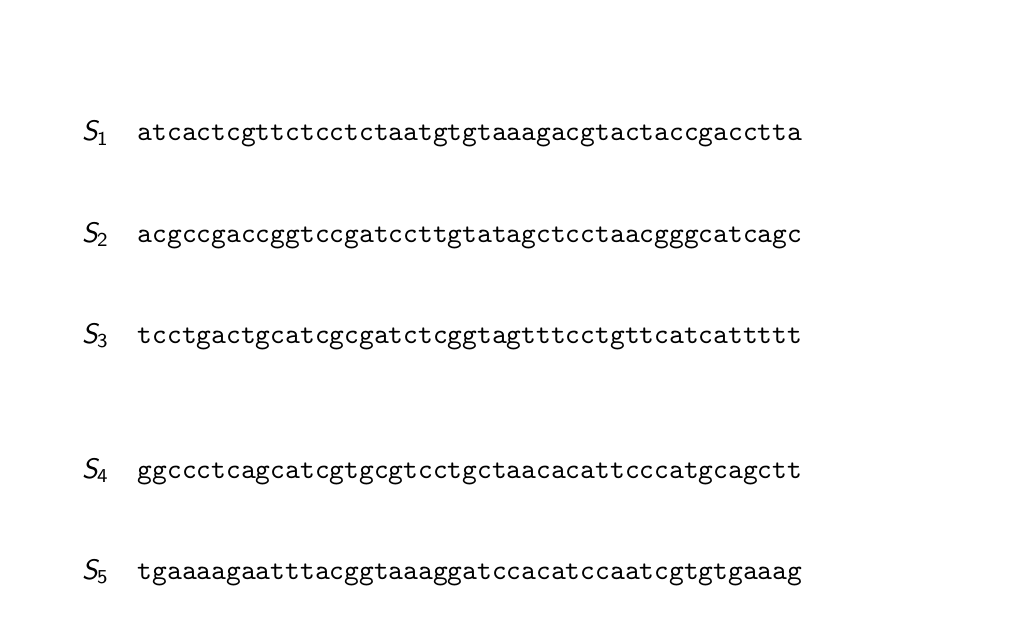
\includegraphics[width=\textwidth]{img/demo0}}
	\only<2>{\centering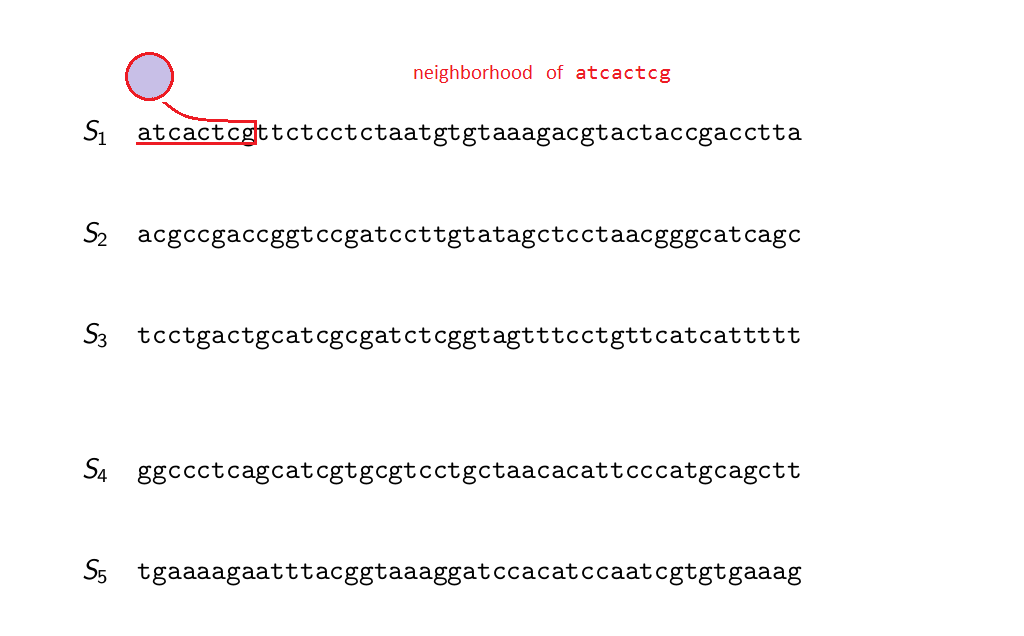
\includegraphics[width=\textwidth]{img/demo1}}
	\only<3>{\centering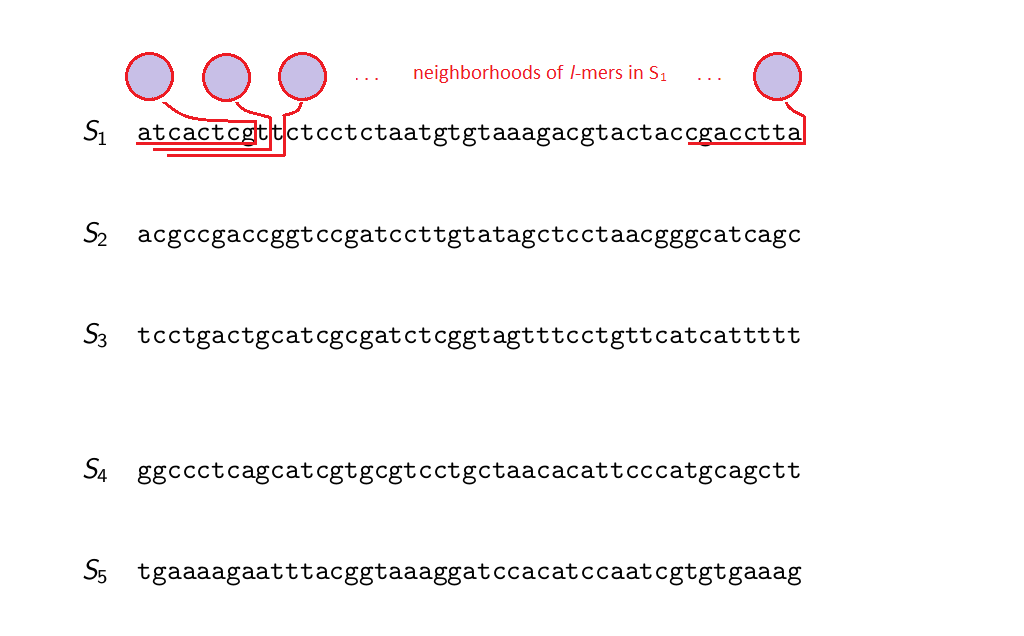
\includegraphics[width=\textwidth]{img/demo2}}
	\only<4>{\centering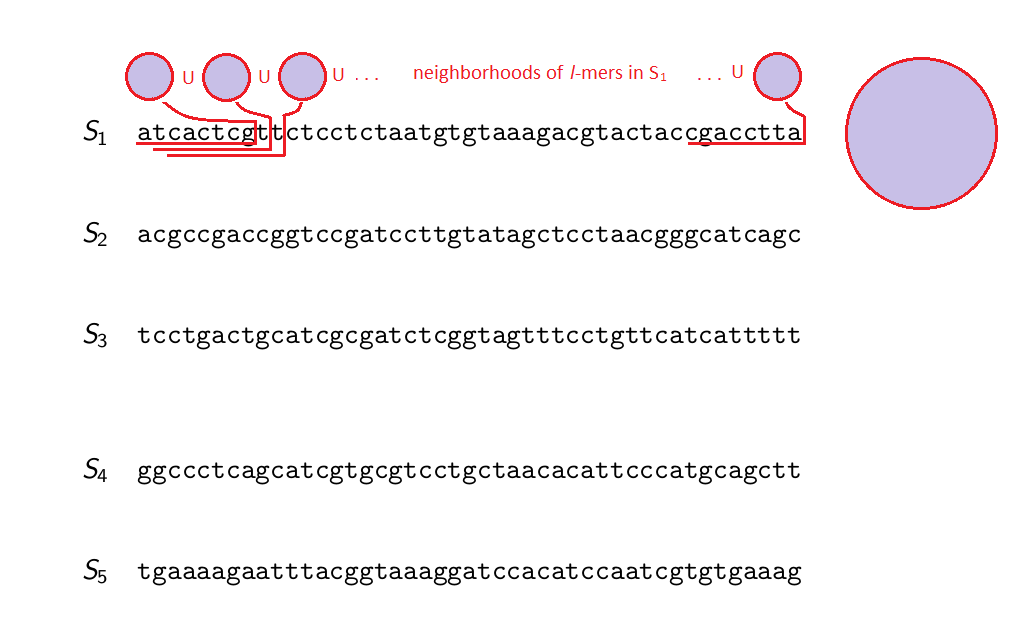
\includegraphics[width=\textwidth]{img/demo3}}
	\only<5>{\centering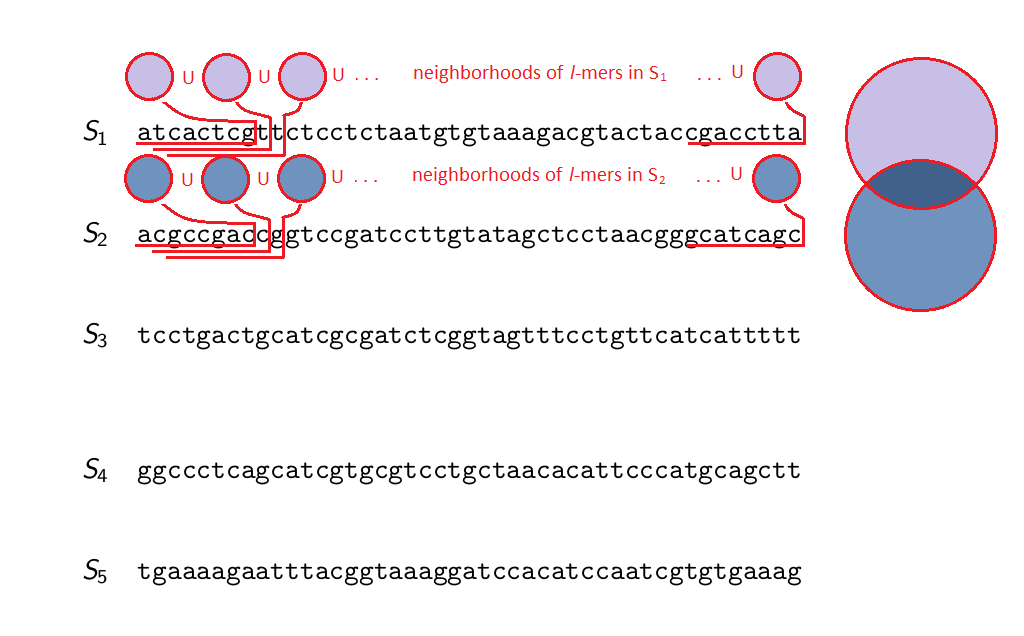
\includegraphics[width=\textwidth]{img/demo4}}
	\only<6>{\centering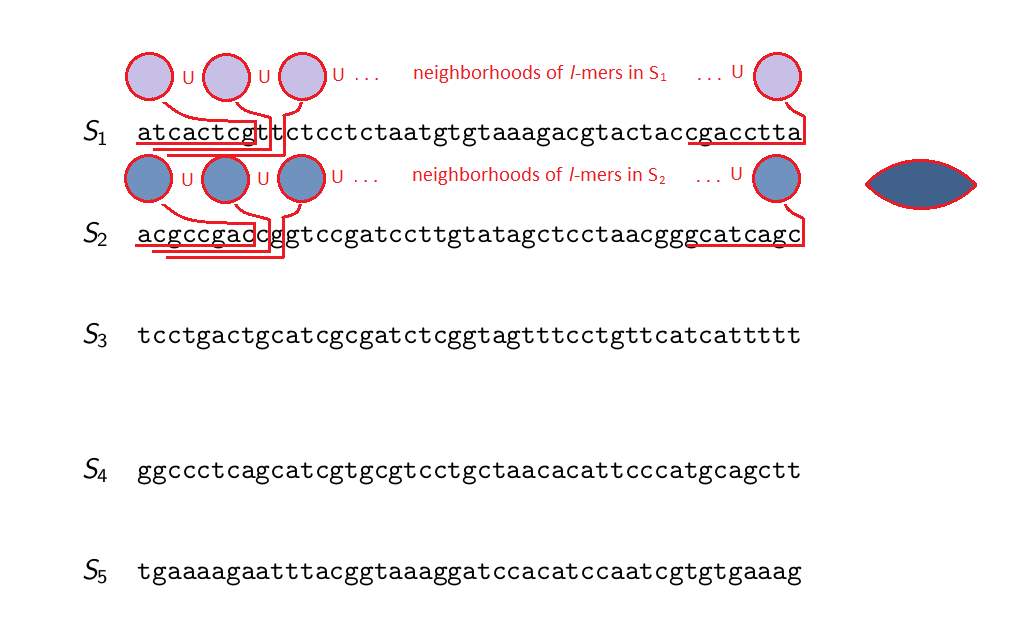
\includegraphics[width=\textwidth]{img/demo5}}
	\only<7>{\centering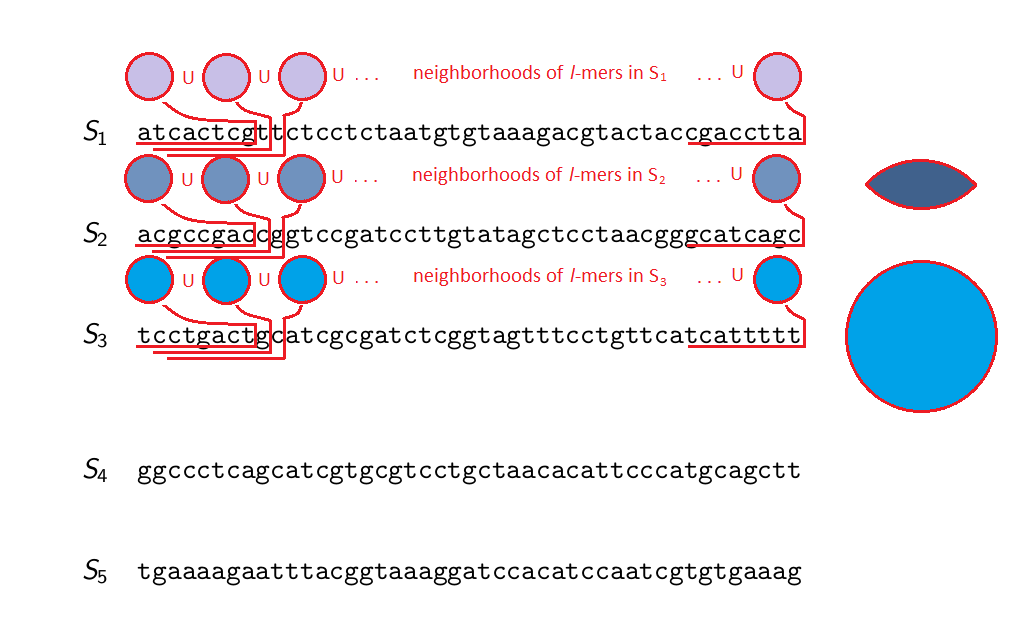
\includegraphics[width=\textwidth]{img/demo6}}
	\only<8>{\centering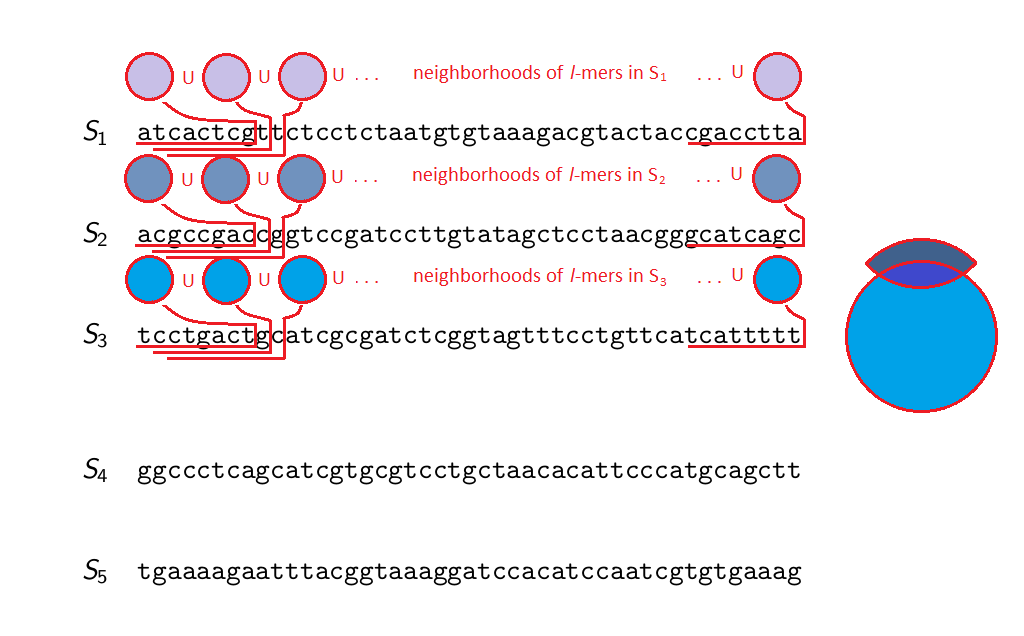
\includegraphics[width=\textwidth]{img/demo7}}
	\only<9>{\centering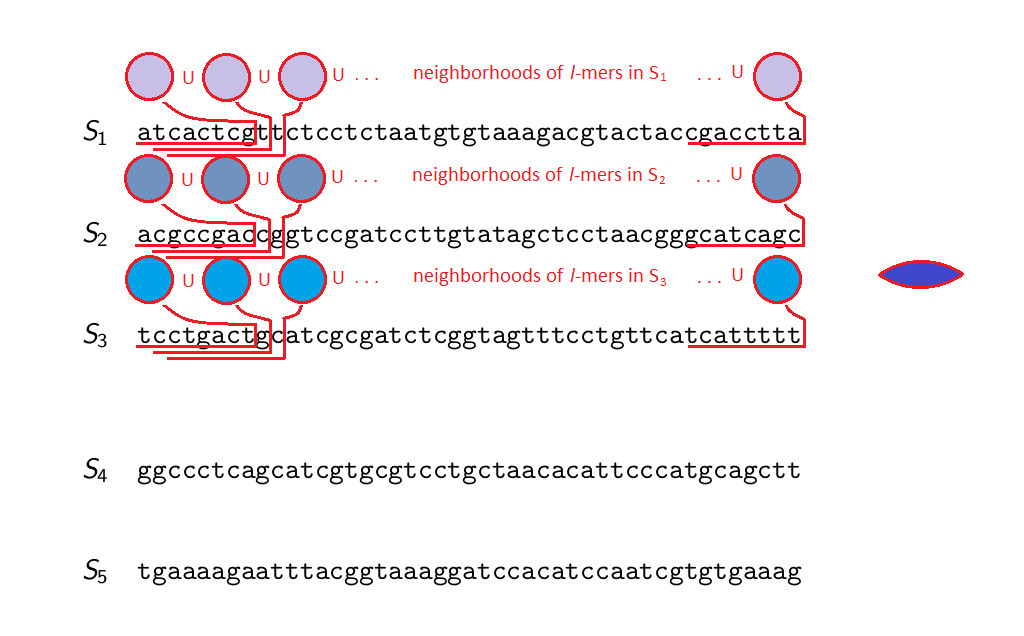
\includegraphics[width=\textwidth]{img/demo8}}
	\end{frame}

\begin{frame}{Representing sets with bits}{EMS-GT}
	\begin{itemize}
	% \item EMS-GT operates on sets of $l$-mers, so efficiently storing these sets is crucial.\\\vspace*{4pt}
	\item ex. the $d$-neighborhood of \texttt{\tcol acgt}, for {\tcol $d$=2} (67 neighbors)\\\vspace*{4pt}
	\end{itemize}
	{\color{black}\texttt{\centering\small\ acgt, \\\vspace*{4pt}
		\ {\red c}cgt, {\red g}cgt, {\red t}cgt, a{\red a}gt, a{\red g}gt, a{\red t}gt,\\
		\ ac{\red a}t, ac{\red g}t, ac{\red t}t, acg{\red a}, acg{\red c}, acg{\red g},\\\vspace*{6pt}
		\ {\red ca}gt, {\red cg}gt, {\red ct}gt, {\red c}c{\red a}t, {\red c}c{\red c}t, {\red c}c{\red t}t, 
		  {\red c}cg{\red a}, {\red c}cg{\red c}, {\red c}cg{\red g},\\
		\ {\red ga}gt, {\red gg}gt, {\red gt}gt, {\red g}c{\red a}t, {\red g}c{\red c}t, {\red g}c{\red t}t, 
		  {\red g}cg{\red a}, {\red g}cg{\red c}, {\red g}cg{\red g},\\
		\ {\red ta}gt, {\red tg}gt, {\red tt}gt, {\red t}c{\red a}t, {\red t}c{\red c}t, {\red t}c{\red t}t, 
		  {\red t}cg{\red a}, {\red t}cg{\red c}, {\red t}cg{\red g},\\
		\ a{\red aa}t, a{\red ac}t, a{\red at}t, a{\red a}g{\red a}, a{\red a}g{\red c}, a{\red a}g{\red g}, 
		  a{\red ga}t, a{\red gc}t, a{\red gt}t,\\
		\ a{\red g}g{\red a}, a{\red g}g{\red c}, a{\red g}g{\red g}, a{\red ta}t, a{\red tc}t, a{\red tt}t, 
		  a{\red t}g{\red a}, a{\red t}g{\red c}, a{\red t}g{\red g},\\
		\ ac{\red aa}, ac{\red ac}, ac{\red ag}, ac{\red ca}, ac{\red cc}, ac{\red cg}, ac{\red ta}, ac{\red tc},
		  ac{\red tg}.\\\vspace*{14pt}
		}
		}
	\end{frame}

\begin{frame}{Representing sets with bits}{EMS-GT}
	\begin{itemize}
	\item<1-> We know there are only {\tcol $4^l$ possible $l$-mers} that can be formed with the DNA bases
		  \{\texttt{a}, \texttt{c}, \texttt{g}, \texttt{t}\};\\\ \\
	\item<2-> thus, EMS-GT can {\tcol represent any set of $l$-mers with $4^l$ bits}:
		\begin{itemize}
		\item set to 1 if the corresponding $l$-mer is a member of the set,
		\item set to 0 otherwise.
		\end{itemize}\ \\\vspace*{7pt}
	\item<3> For efficiency, EMS-GT stores the $4^l$ bits as {\tcol $\frac{4^l}{32}$ 32-bit integers}.
	\end{itemize}
	\end{frame}

\begin{frame}{Representing sets with bits}{EMS-GT}
	\begin{itemize}
	\item ex. the $d$-neighborhood of \texttt{\tcol acgt}, for {\tcol $d$=2} (67 neighbors)\\\vspace*{4pt}
	\item<2-> {\tcol $l$=4} 
		\uncover<3->{$\ \rightarrow\ $ $4^l$ = {\tcol 256 possible $l$-mers}}
		\uncover<4->{$\ \rightarrow\ $ $\frac{4^l}{32}=${\tcol\ 8 32-bit integers}}
	\end{itemize}
	\only<1>{\color{black}\texttt{\centering\small\ acgt, \\\vspace*{4pt}
		\ {\red c}cgt, {\red g}cgt, {\red t}cgt, a{\red a}gt, a{\red g}gt, a{\red t}gt,\\
		\ ac{\red a}t, ac{\red g}t, ac{\red t}t, acg{\red a}, acg{\red c}, acg{\red g},\\\vspace*{6pt}
		\ {\red ca}gt, {\red cg}gt, {\red ct}gt, {\red c}c{\red a}t, {\red c}c{\red c}t, {\red c}c{\red t}t, 
		  {\red c}cg{\red a}, {\red c}cg{\red c}, {\red c}cg{\red g},\\
		\ {\red ga}gt, {\red gg}gt, {\red gt}gt, {\red g}c{\red a}t, {\red g}c{\red c}t, {\red g}c{\red t}t, 
		  {\red g}cg{\red a}, {\red g}cg{\red c}, {\red g}cg{\red g},\\
		\ {\red ta}gt, {\red tg}gt, {\red tt}gt, {\red t}c{\red a}t, {\red t}c{\red c}t, {\red t}c{\red t}t, 
		  {\red t}cg{\red a}, {\red t}cg{\red c}, {\red t}cg{\red g},\\
		\ a{\red aa}t, a{\red ac}t, a{\red at}t, a{\red a}g{\red a}, a{\red a}g{\red c}, a{\red a}g{\red g}, 
		  a{\red ga}t, a{\red gc}t, a{\red gt}t,\\
		\ a{\red g}g{\red a}, a{\red g}g{\red c}, a{\red g}g{\red g}, a{\red ta}t, a{\red tc}t, a{\red tt}t, 
		  a{\red t}g{\red a}, a{\red t}g{\red c}, a{\red t}g{\red g},\\
		\ ac{\red aa}, ac{\red ac}, ac{\red ag}, ac{\red ca}, ac{\red cc}, ac{\red cg}, ac{\red ta}, ac{\red tc},
		  ac{\red tg}.\\\vspace*{14pt}
		}
		}
	\only<2-4>{ \centering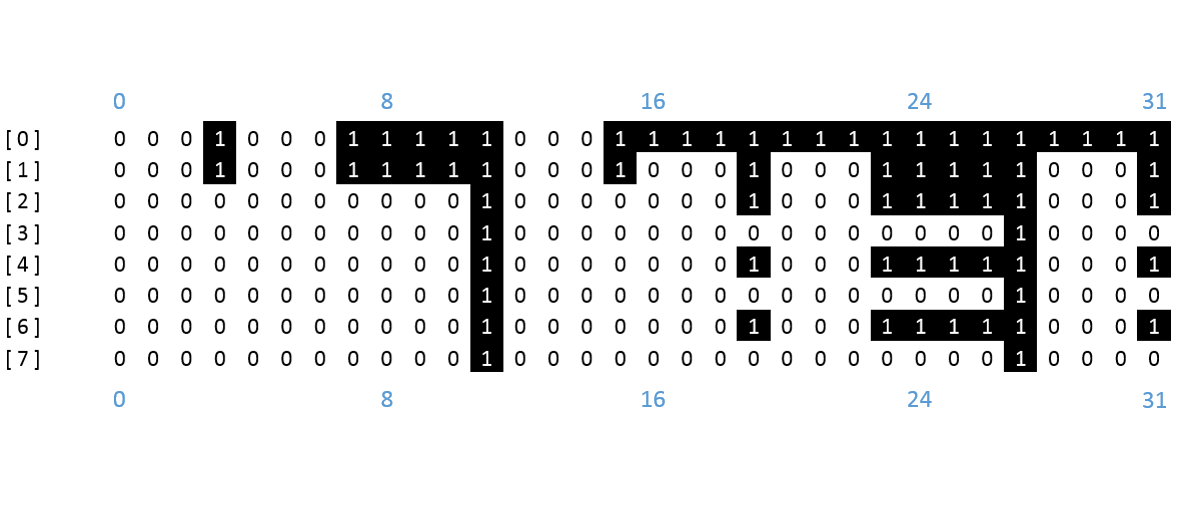
\includegraphics[width=\textwidth]{img/acgt1.png}\\ }
	\only<5>{ \centering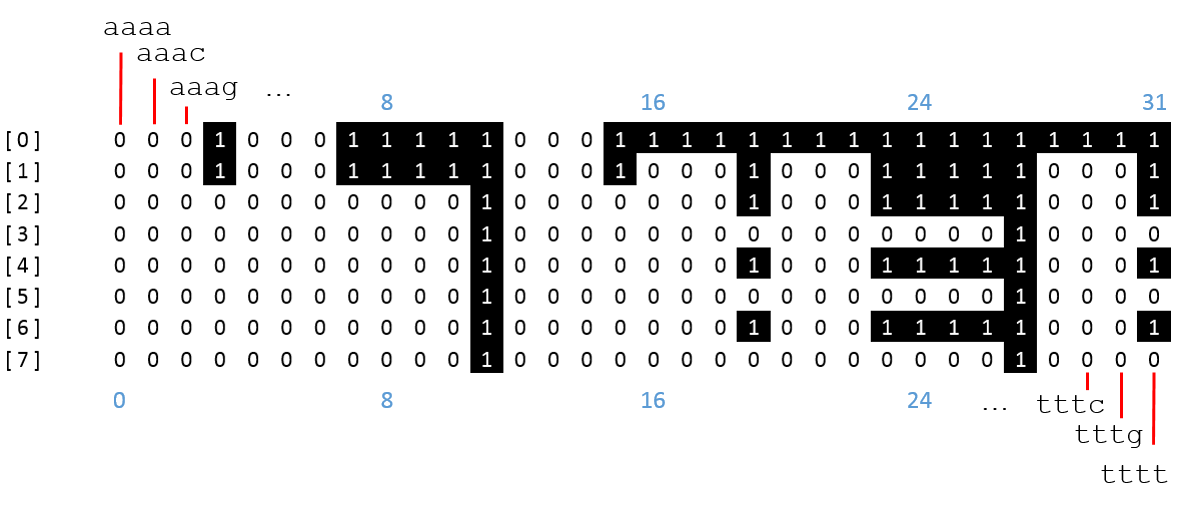
\includegraphics[width=\textwidth]{img/acgt2.png}\\ }
	\only<6>{ \centering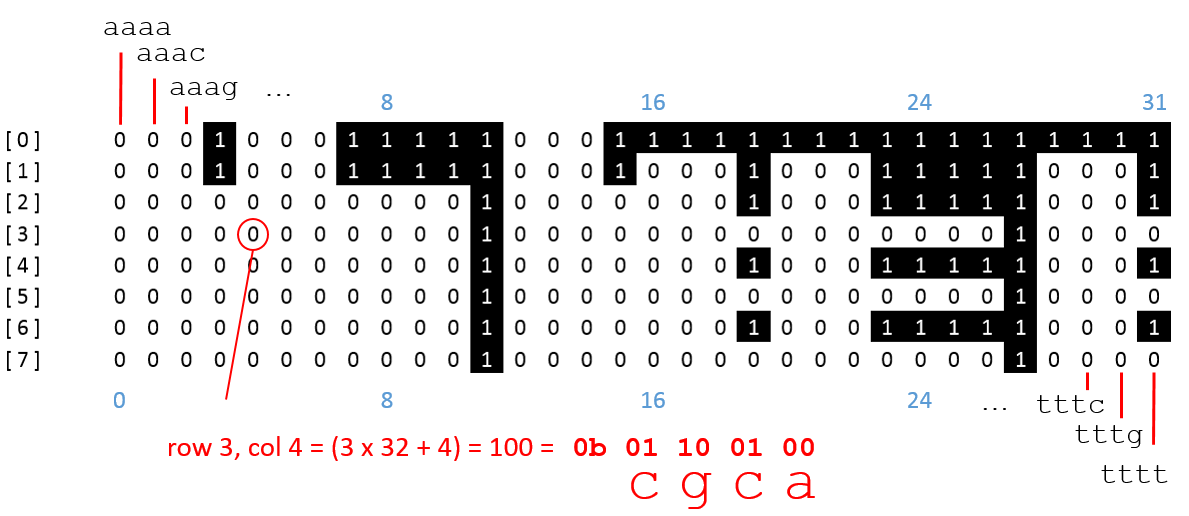
\includegraphics[width=\textwidth]{img/acgt3.png}\\ }
	\end{frame}

\begin{frame}{Building neighborhoods in blocks}{EMS-GT}
	\color{black}
	{\centering Given the {\tcol neighborhood bit-array $N_x$} for $l$-mer $x$,\\\vspace*{4pt}
		if we partition $N_x$ into {\tcol blocks of $4^k$ bits each}, $k < l$, \\\vspace*{4pt}
		% the $l$-mers in a block all begin with the same {\tcol prefix (length $l$-$k$)},\\\vspace*{4pt}
		each block conforms to one of {\tcol ($k + 2$) patterns}.\\\ \\\ \\
		}
	
	\uncover<2>{\centering ex. patterns in $\tcol N_\texttt{acgtacgtacgt}$ for {\tcol $k$=5} %\\\vspace*{4pt}
		\small$\ \rightarrow\ \tcol4^5$\tcol=32$\times$32 bits per block\\\vspace*{14pt}
		\begin{columns}
		\scriptsize\centering
		\begin{column}{.135\textwidth}\centering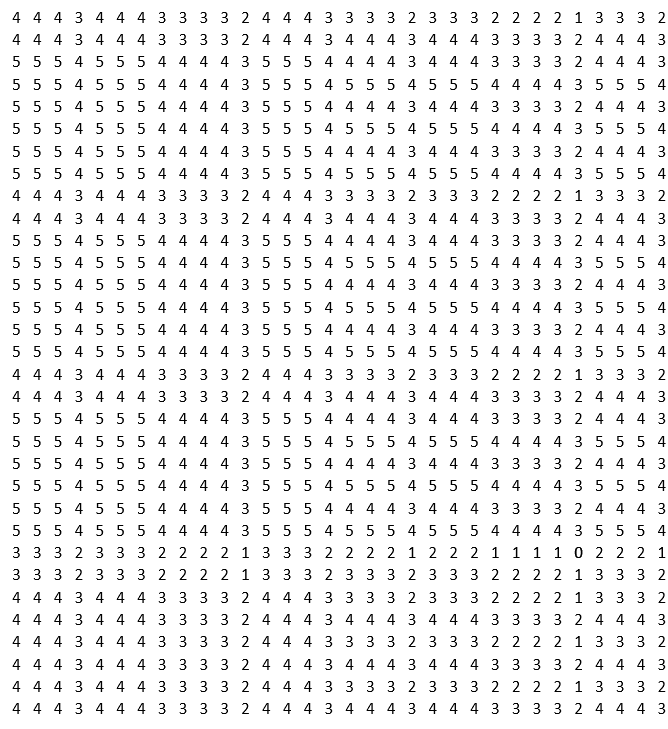
\includegraphics[width=0.98\textwidth]{img/-1}\\Pattern -1\end{column}
		\begin{column}{.135\textwidth}\centering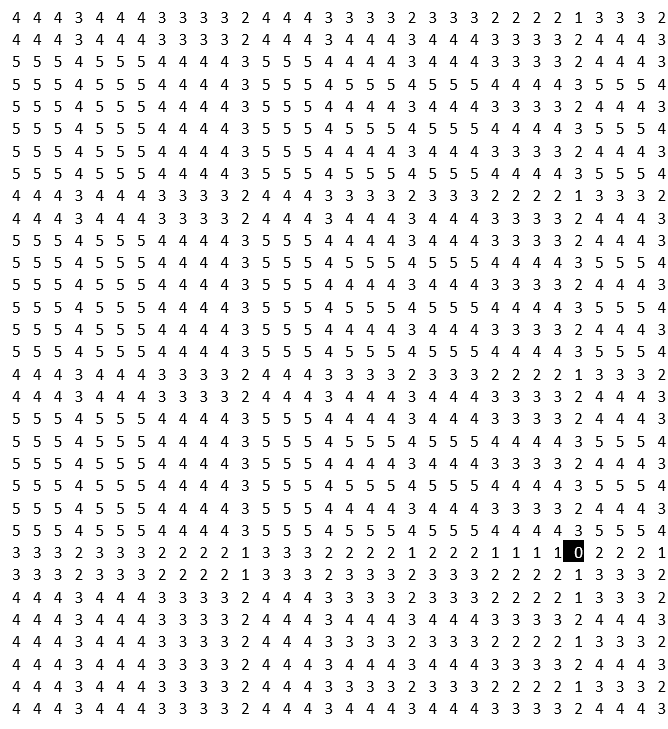
\includegraphics[width=0.98\textwidth]{img/0}\\Pattern 0 \end{column} 
		\begin{column}{.135\textwidth}\centering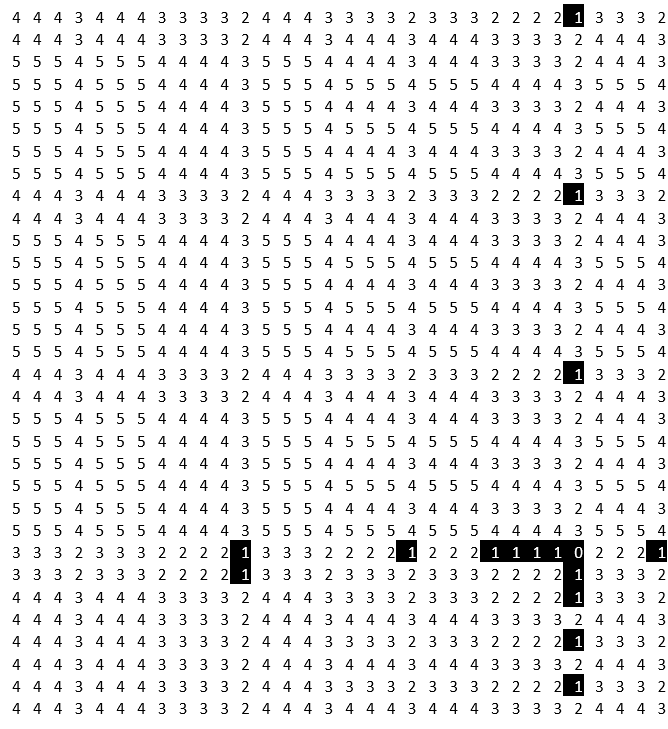
\includegraphics[width=0.98\textwidth]{img/1}\\Pattern 1 \end{column}
		\begin{column}{.135\textwidth}\centering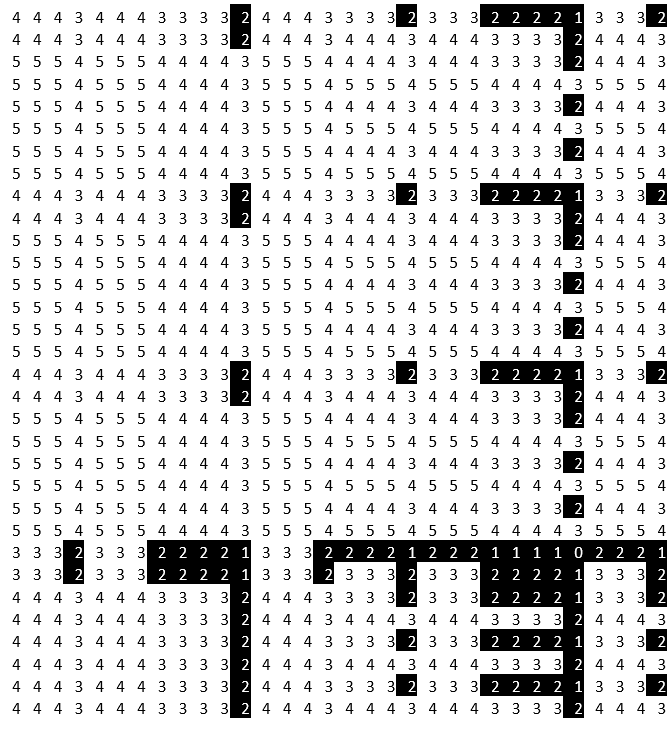
\includegraphics[width=0.98\textwidth]{img/2}\\Pattern 2 \end{column}
		\begin{column}{.135\textwidth}\centering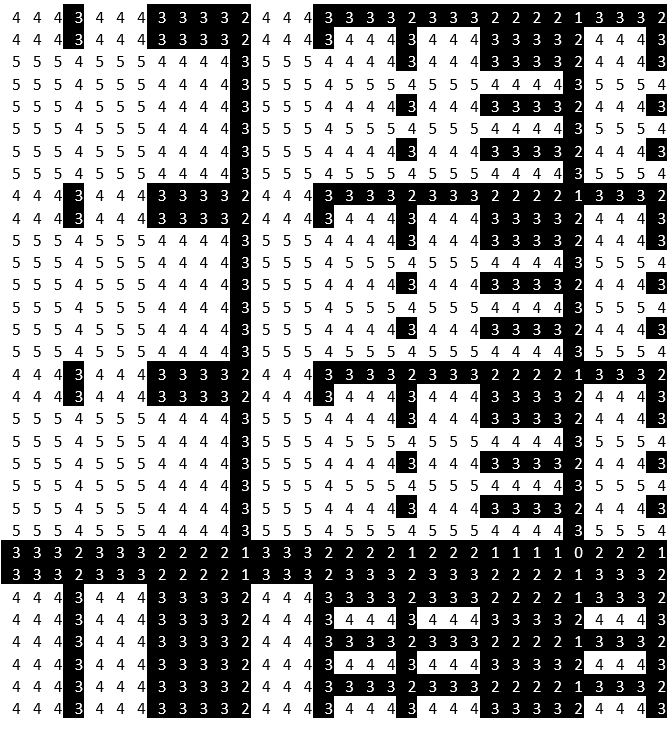
\includegraphics[width=0.98\textwidth]{img/3}\\Pattern 3 \end{column}
		\begin{column}{.135\textwidth}\centering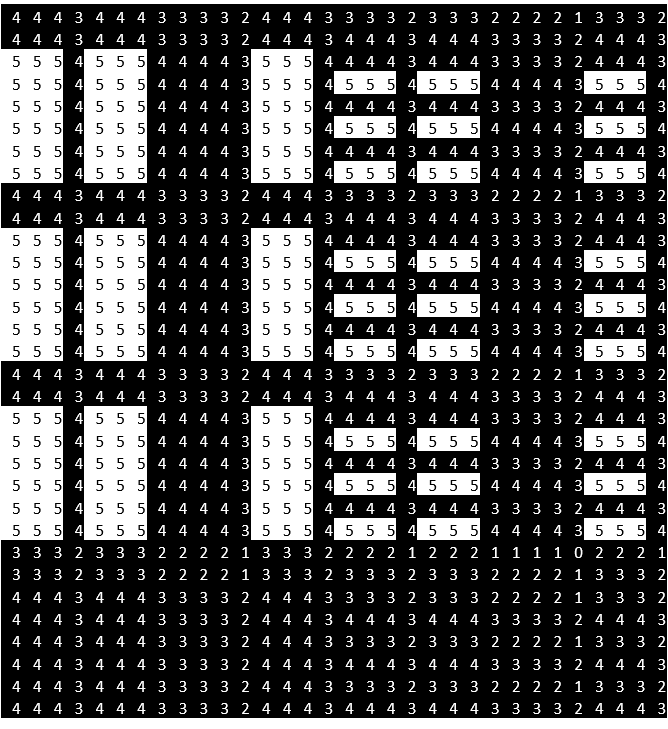
\includegraphics[width=0.98\textwidth]{img/4}\\Pattern 4 \end{column}
		\begin{column}{.135\textwidth}\centering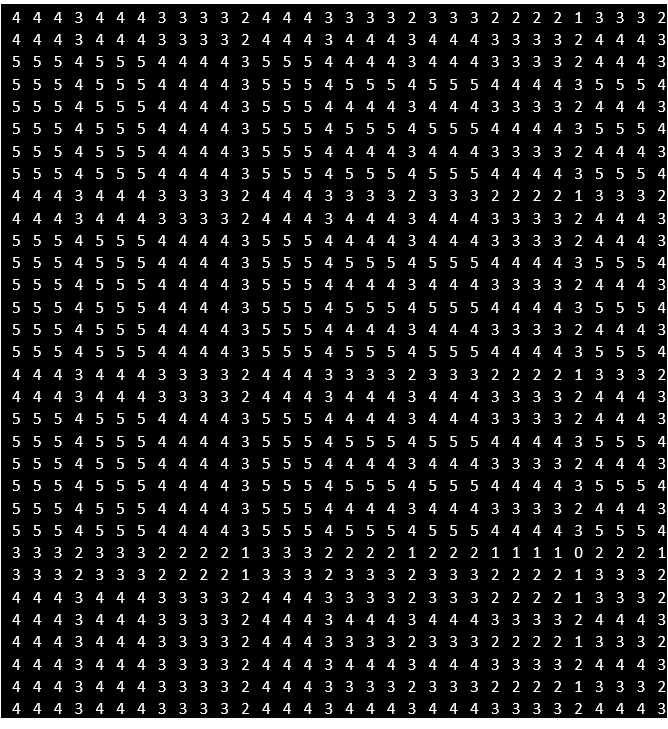
\includegraphics[width=0.98\textwidth]{img/5}\\Pattern 5 \end{column}
		\end{columns}\ \\\ \\
		}

	\end{frame}

\begin{frame}{Building neighborhoods in blocks}{EMS-GT}
	\begin{itemize}
		\item {\bf prefix} = first ($l$-$k$) characters, {\tcol $k$-suffix} = last $k$ characters\\ %\vspace*{4pt}
		
		\begin{columns}
		\centering
		\begin{column}{4.0cm}
			\begin{flushright}
			\texttt{\large {\bf acgtaaa}{\tcol aaaaa} $\rightarrow$}\vspace*{4.0cm}\\\ \\
			\end{flushright}
			\end{column}
		\begin{column}{4.0cm}
			\ \\\centering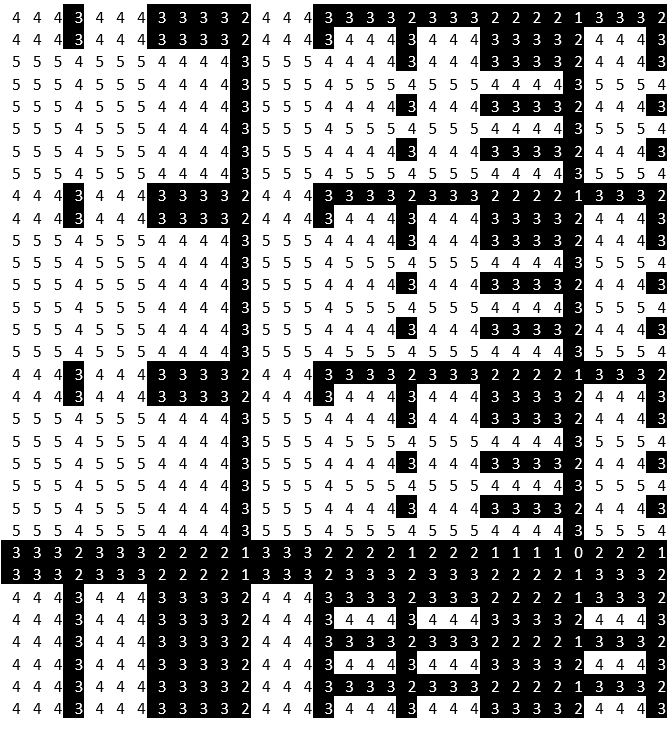
\includegraphics[width=4.0cm]{img/3.png}
			\end{column}
		\begin{column}{4.0cm}
			\ \vspace*{3.8cm}\\\vspace*{4pt}$\leftarrow$ \texttt{\large {\bf acgtaaa}{\tcol ttttt}}
			\end{column}
		\end{columns}

		\item due to the alphabetical ordering, $l$-mers in the same block all {\tcol have the same prefix}, and {\tcol differ only in their $k$-suffixes}\\\vspace*{4pt}
		\end{itemize}
	\end{frame}

\begin{frame}{Building neighborhoods in blocks}{EMS-GT}
	\color{black}
	For the neighborhood $N_x$ of $l$-mer $x$,\\\ \\
	\begin{itemize}
	\item $x$'s {\bf prefix} determines which patterns apply to which blocks;\\\ \\
	\item $x$'s {\tcol $k$-suffix} determines the structure of the patterns\\\ \\
	\end{itemize}
	\end{frame}

\begin{frame}{Building neighborhoods in blocks}{EMS-GT}
	\begin{columns}[c]
		\centering
		\begin{column}{6.0cm}
		\begin{itemize}
			\item ex. $d$=5, $k$=5\\\vspace*{4pt}
			$x$ = \texttt{\LARGE{acgtacg}{\tcol tacgt}}\\\ \\
			\only<1>{\ \\
				\item color map: number of mismatches from $x$'s suffix \texttt{\tcol tacgt} 
				of all possible $k$-suffixes\\\ \\\ \\
				}
			\only<2>{
				\item if prefix = \texttt{\LARGE{\red cgac}a{\red tc}}\\
				({\red 6 mismatches} from \texttt{acgtacg})\\\ \\
				\item we cannot use any $k$-suffix to form a neighbor of $x$\\ \ 
				}
			\only<3>{
				\item if prefix = \texttt{\LARGE a{\red gac}a{\red tc}}\\
				({\red 5 mismatches} from  \texttt{acgtacg})\\\ \\
				\item adding the $k$-suffix \texttt{\tcol tacgt}\\
				forms a neighbor of $x$\\\ \\
				}
			\only<4>{
				\item if prefix = \texttt{\LARGE a{\red gac}a{\red t}g}\\
				({\red 4 mismatches} from  \texttt{acgtacg})\\\ \\
				\item any $k$-suffix with up to\\
				{\tcol 1 mismatch} from \texttt{\tcol tacgt}\\
				forms a neighbor of $x$
				}
			\only<5>{
				\item if prefix = \texttt{\LARGE a{\red ga}ta{\red t}g}\\
				({\red 3 mismatches} from  \texttt{acgtacg})\\\ \\
				\item any $k$-suffix with up to\\
				{\tcol 2 mismatches} from \texttt{\tcol tacgt}\\
				forms a neighbor of $x$
				}
			\only<6>{
				\item if prefix = \texttt{\LARGE ac{\red a}ta{\red t}g}\\
				({\red 2 mismatches} from  \texttt{acgtacg})\\\ \\
				\item any $k$-suffix with up to\\
				{\tcol 3 mismatches} from \texttt{\tcol tacgt}\\
				forms a neighbor of $x$
				}
			\only<7>{
				\item if prefix = \texttt{\LARGE ac{\red a}tacg}\\
				({\red 1 mismatch} from  \texttt{acgtacg})\\\ \\
				\item any $k$-suffix with up to\\
				{\tcol 4 mismatches} from \texttt{\tcol tacgt}\\
				forms a neighbor of $x$
				}
			\only<8>{
				\item if prefix = \texttt{\LARGE acgtacg}\\
				({\red 0 mismatches}, $x$'s actual prefix)\\\ \\
				\item any $k$-suffix forms a neighbor of $x$, 
				since all $k$-suffixes have at most {\tcol 5 mismatches} from \texttt{\tcol tacgt}\\
				}
			\end{itemize}

		\end{column}
		\begin{column}{6.0cm}
		\only<1>{\centering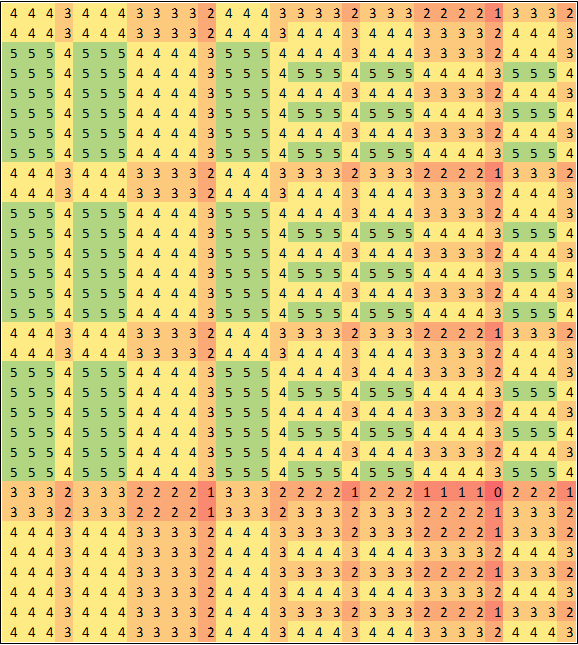
\includegraphics[width=6.0cm, height=6.45cm]{img/D(tacgt)}\\}
		\only<2>{\centering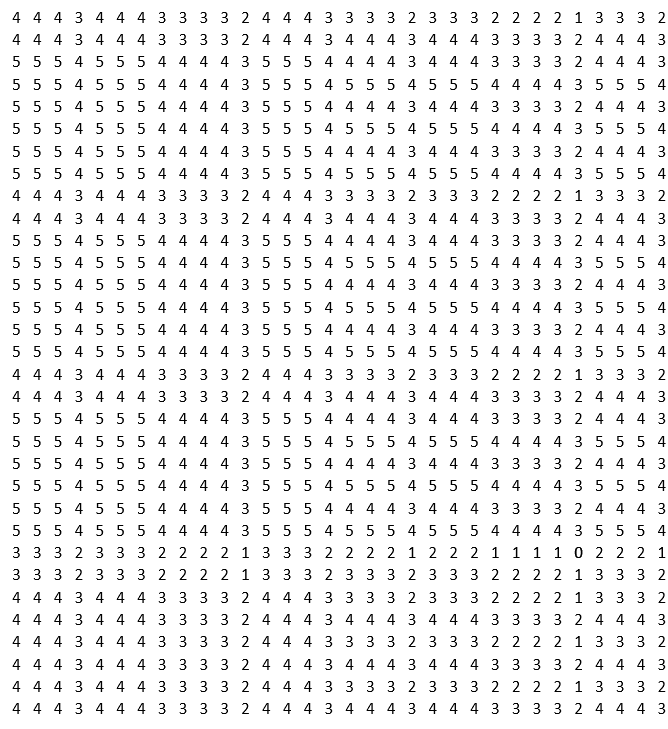
\includegraphics[width=6.0cm]{img/-1}\\}
		\only<3>{\centering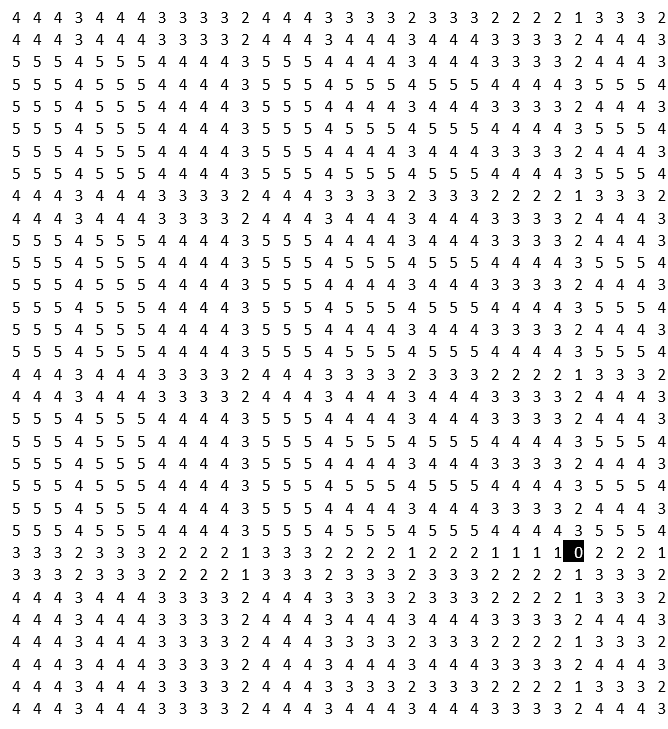
\includegraphics[width=6.0cm]{img/0}\\}
		\only<4>{\centering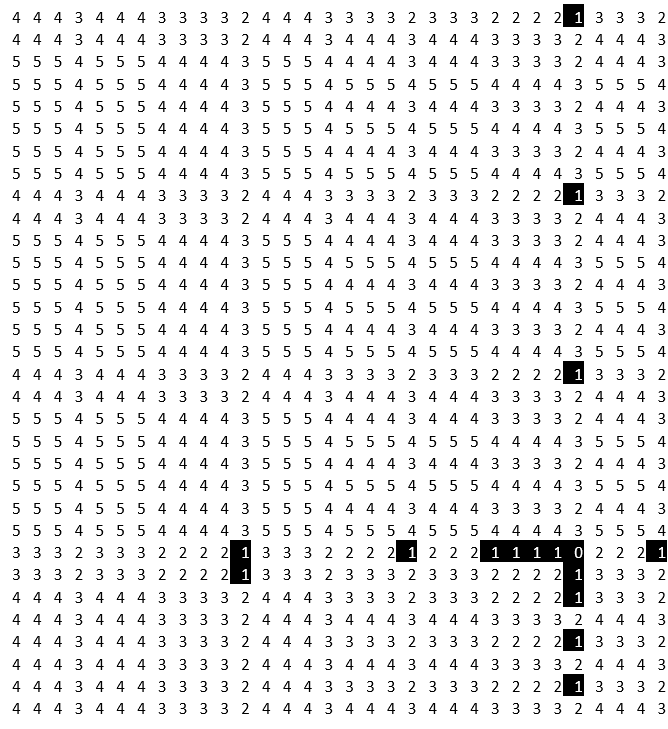
\includegraphics[width=6.0cm]{img/1}\\}
		\only<5>{\centering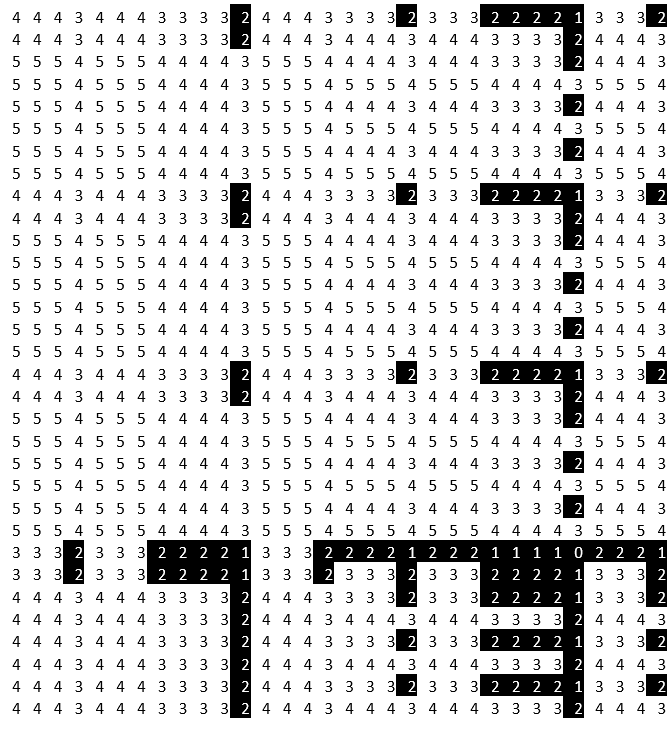
\includegraphics[width=6.0cm]{img/2}\\}
		\only<6>{\centering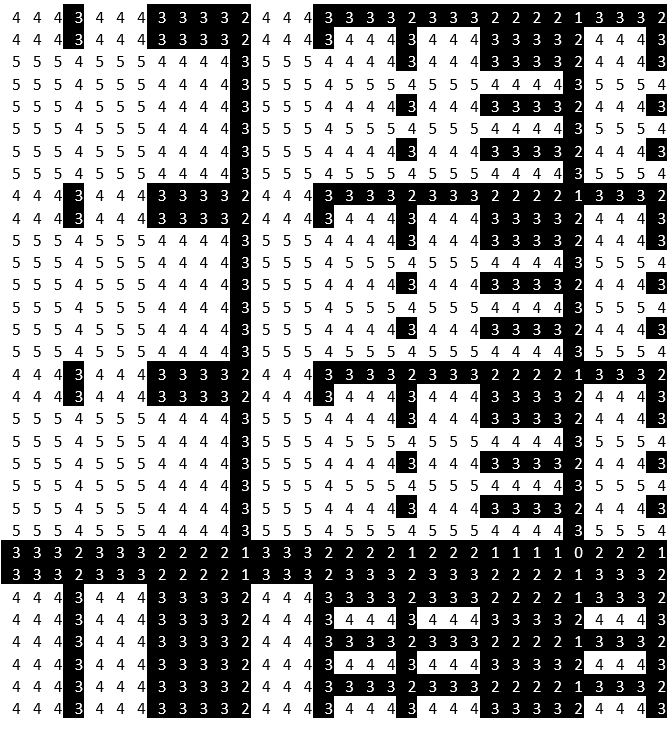
\includegraphics[width=6.0cm]{img/3}\\}
		\only<7>{\centering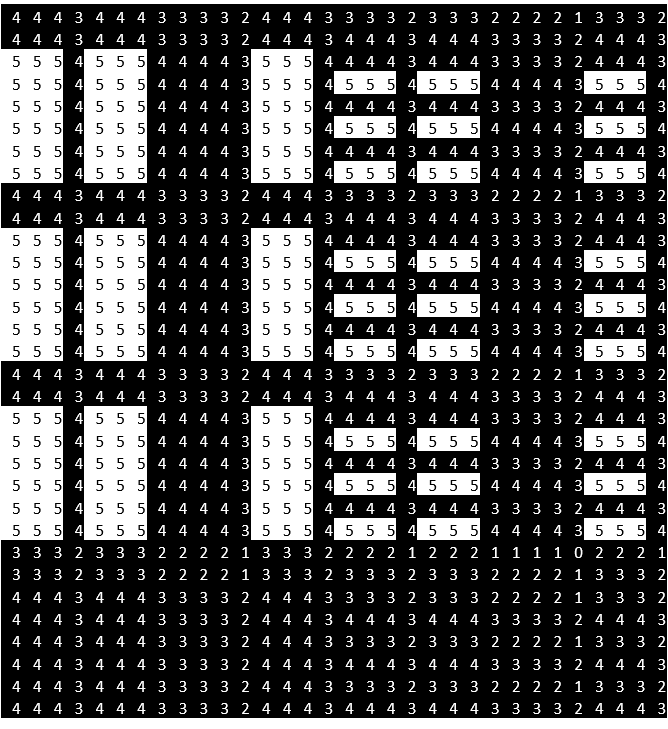
\includegraphics[width=6.0cm]{img/4}\\}
		\only<8>{\centering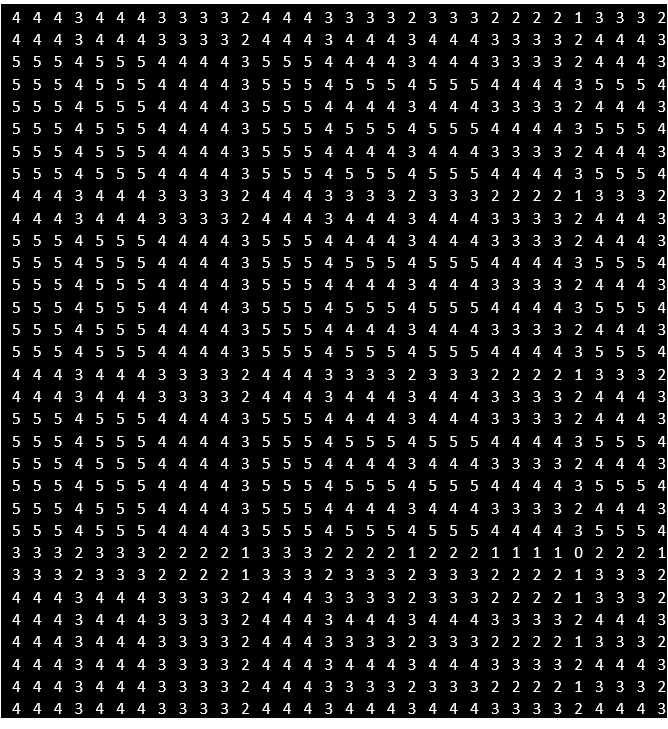
\includegraphics[width=6.0cm]{img/5}\\}
		\end{column}
		\end{columns}
	\end{frame}

\begin{frame}{Performance}{EMS-GT}
	\centering
	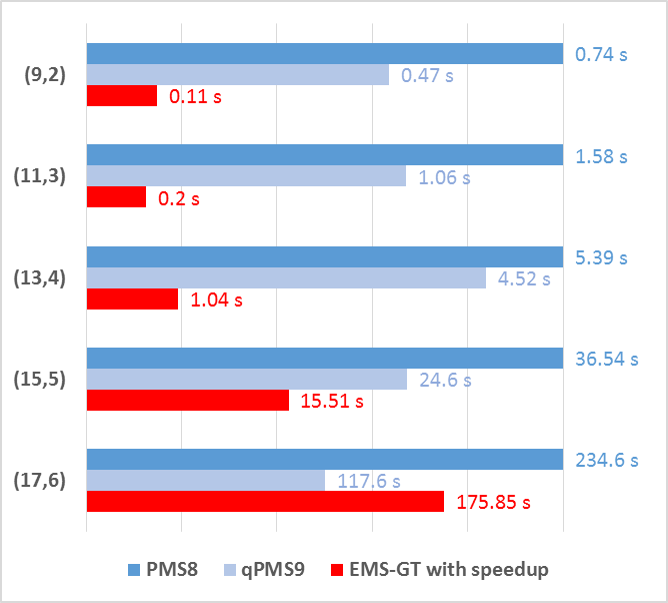
\includegraphics[width=0.8\textwidth]{img/emsgt-with-speedup-vs-PMS,qPMS9.png}\\
	\end{frame}

\end{document}